\hypersetup{pdfborder=0 0 0}


%-------------------------------------------------------------------------------------
\section{Comparison of solitary waves and associated signal from in situ data}
\label{sectionCampagne}

This section presents some measurements made during the field campaign Gibraltar 2020, .     Section gives a brief overview of the water masses from the sampling. Section

\subsection{Field campaign Gibraltar 2020 overview}
A field campaign of in situ measurements was carried out by SHOM (and other labs) in fall 2020 in the Strait of Gibraltar (and west Alboran) aboard research and survey ship L'Atalante. On site measures were taken on site by ship-based instruments from 8/10/2020 to 20/10/2020. Among those, sampling of the water column at both end of the Strait were realized: at eastern end the 14th and 15th october, and west of the Strait the 16th of october.

Additionally, five moorings were deployed as presented in table \ref{tab_moor}, there locations are also indicated in figure \ref{fig_moor}. Three of the moorings, M1, M3 and M5, are equipped with CTD sensors, the other two, M2 and M4, with ADCP sensors. Sampling frequency range from tens of seconds to one minute.

The measures from moorrings that are analyzed/compared to simulated processes here are from the period covering 8/10 to 18/10 when both types of moorings were available, and only concern data from M2, M4 and M5.


\begin{table}[!h]
        \centering
        \begin{tabular}{|c|c|c|c|}
                \hline
                 & type & position(deg minute) & time \\ 
                 \hline
                M1 & hydro & N35 55.264 W005 46.739 & 8/10/2020 15h - 9/11/2020 12h\\
                M2 & couranto & N35 55.761 W005 45.288 & 8/10/2020 5h - 17/10/2020 15h\\
                M3 & hydro & N35 54.719 W005 44.459 & 8/10/2020 13h - 22/10/2020 21h\\
                M4 & couranto & N35 55.870 W005 41.020 & 8/10/2020 7h - 17/10/2020 14h\\
                M5 & hydro & N35 56.229 W005 41.026 & 8/10/2020 9h - 1/11/2020 14h\\
                \hline
        \end{tabular}
        \captionof{table}{Type of measures, coordinates and date of deployment for moorings of Gibraltar 2020 field campaign.}
        \label{tab_moor}
        %\end{minipage}
\end{table}


\begin{figure}[!h]
% \centering
 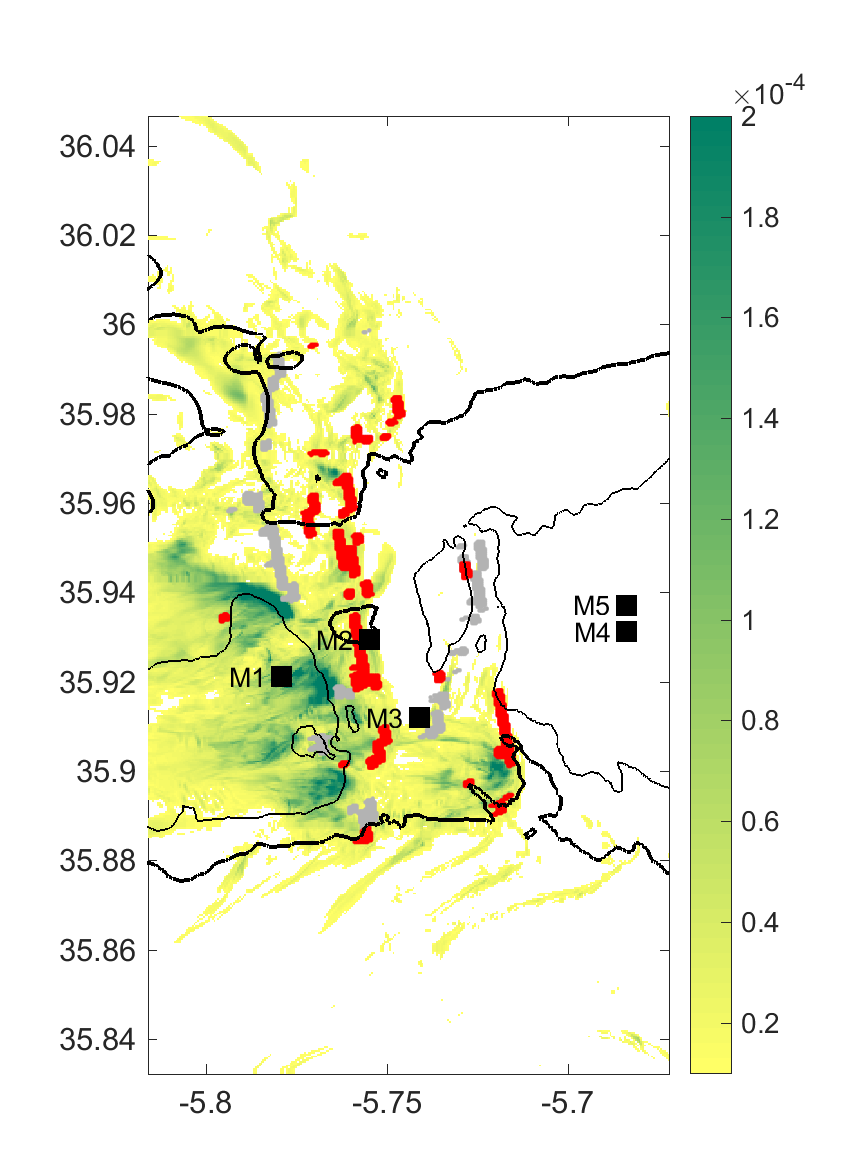
\includegraphics[width=0.4\textwidth]{./GBR3D/Fig_Moor.png}
 \caption {Locations of moorings deployed during Gibraltar 2020 (squares and triangles, over map of standard deviation of parameter Q (colorbar) and location of hydraulic jump of w-type and s-type from high-resolution numerical modelling of the Strait of Gubraltar, as presented in section \ref{sectionSim3D}.}
 \label{fig_moor}
\end{figure}


\subsection{Insights from VHR simulation as help in preparation of Gibraltar 2020}

The simulatios presented in section \ref{sectionSim3D} were a help in preparation of the field campaign.  

To compose with restrictions linked to the dense maritime traffic of the area, and restriction of the measure/ in regard to the strong currents of the Strait and steep slopes for moorings and water column samplings.

Choice of sampling frequency. As presented in the field of standard deviation of parameter Q in figure \ref{fig_moor}, M1 was positioned down western slope of the sill downflow of a potential primary instability generation area (see section \ref{PartDiag3D} and \ref{section3DResFlow} for a discussion of this diagnosis).


Propagation of solitary waves in the non-hydrostatic high-resolution model is esteeemed to be accurate, see for exemple figure ... that compares with (simulationtime). The form of the the wave train can still differ. (METTRE COMP SAR)


The speed of propagation of the ISW was used to predict position of ISW in relation to the tidal cycle as precdicted by harmonic prediction  (not shown). It was accurate at least in the Strait of Gibraltar itself. In the Alboran Sea, where the influence of the gyre is great on the form of the wave packet, prediction was not as accurate. 


Additionally and as presented in section \ref{section_sim_moor}, simulated mooring data (HF outputs at coordinated) helps understand signal observed.



(Ajouter dans papier 3D : important for high resolution bathymetry at camarinal since flow over and effect of vertical compression /conservation of flux on barotropic currents that command the transition from sub to supercritical and thus the existence and form of hyd jump, especially for variety of regimen between super strong tide and neap tide weak where no jump



\subsection{General points of circulation in the Strait during observation period}

Juste metre les WM et dire que a la gyre, voit les images SST l'upwelling qui s'affaiblit sur période où était.  tout renversé, type d'outflow à M2)

The west Alboran Gyre was present in the West Alboran Sea (not shown) during the field campaign. 




The in situ timeperiod covers one (for ship-based and ADCP moorings) or two (for CTD moorings) neap-spring tide cycle. Figure ... shows the depth-averaged zonal component of current measures at Camarinal Sill from M2 data. The beginning of measures are during the neap tide part of the cycle.


Figure ... presents the $\theta$-S diagram from , with each color corresponding to a different sampling station.
West, no med waters were sampled at the northenmost (ou si mais tres melange... va pas loin sur diagramme vers la bas... max salinity est 36.33) and southernmost station. East in med waters find less signal of LIW for southern station.


\subsection{Observations of solitary waves and currents at Camarinal Sill}
\label{section_obs_moor}

\begin{figure}[!h]
% \centering
 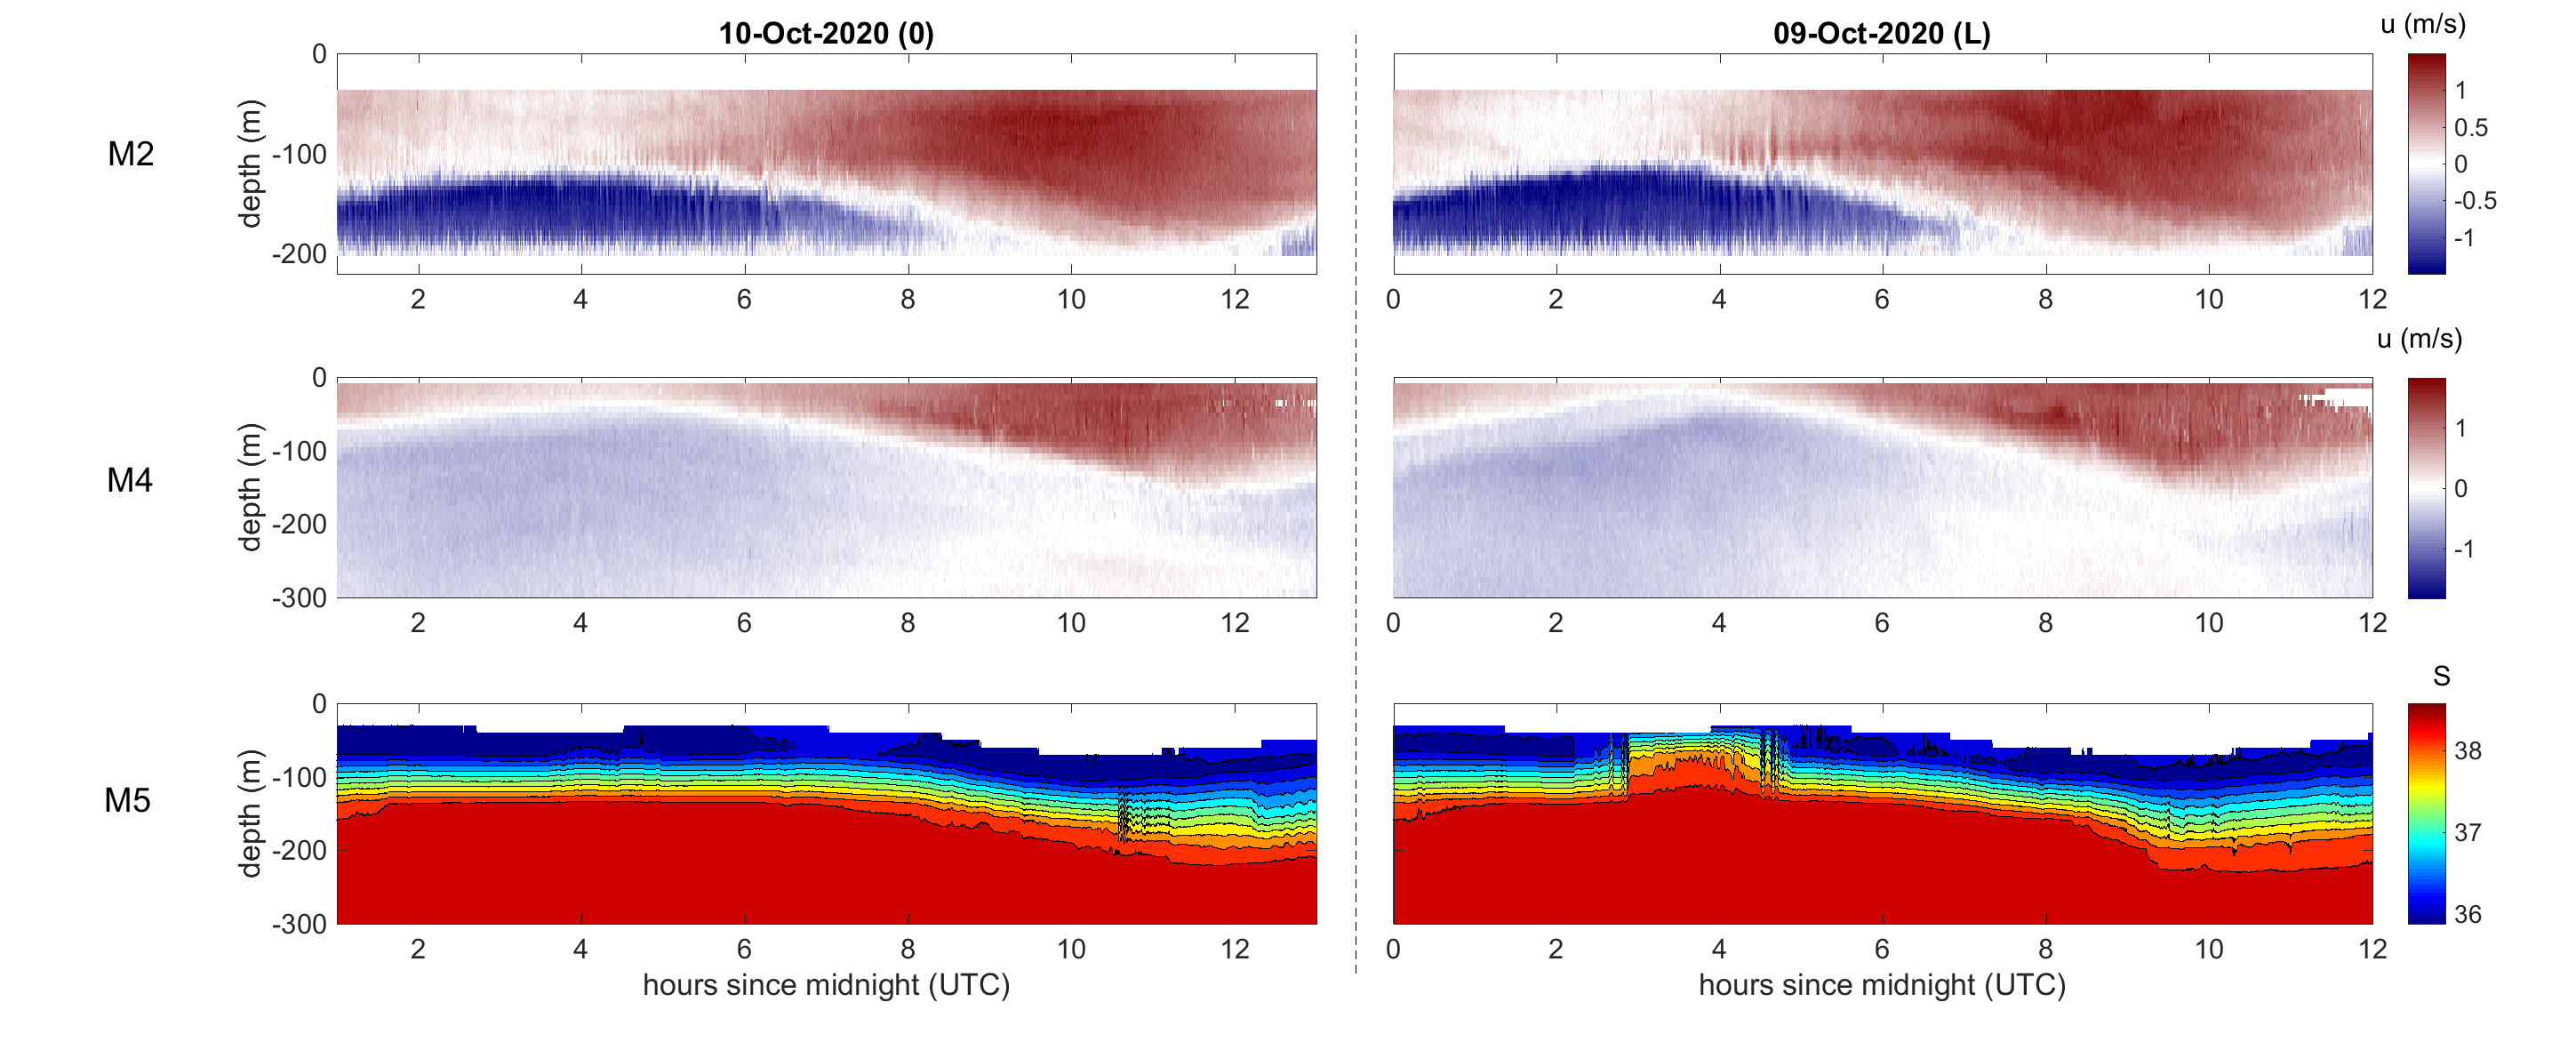
\includegraphics[width=\textwidth]{./GBR3D/US_moorings1.png}
 \caption {Timeseries of moorings data over the water column from M2 (upper row), M4 (center row) and M5 (lower row). The zonal component of currents is represented for M2 and M4 data, and the measured salinity for M5 data.}
 \label{fig_moor_US1}
\end{figure}

\begin{figure}[!h]
% \centering
 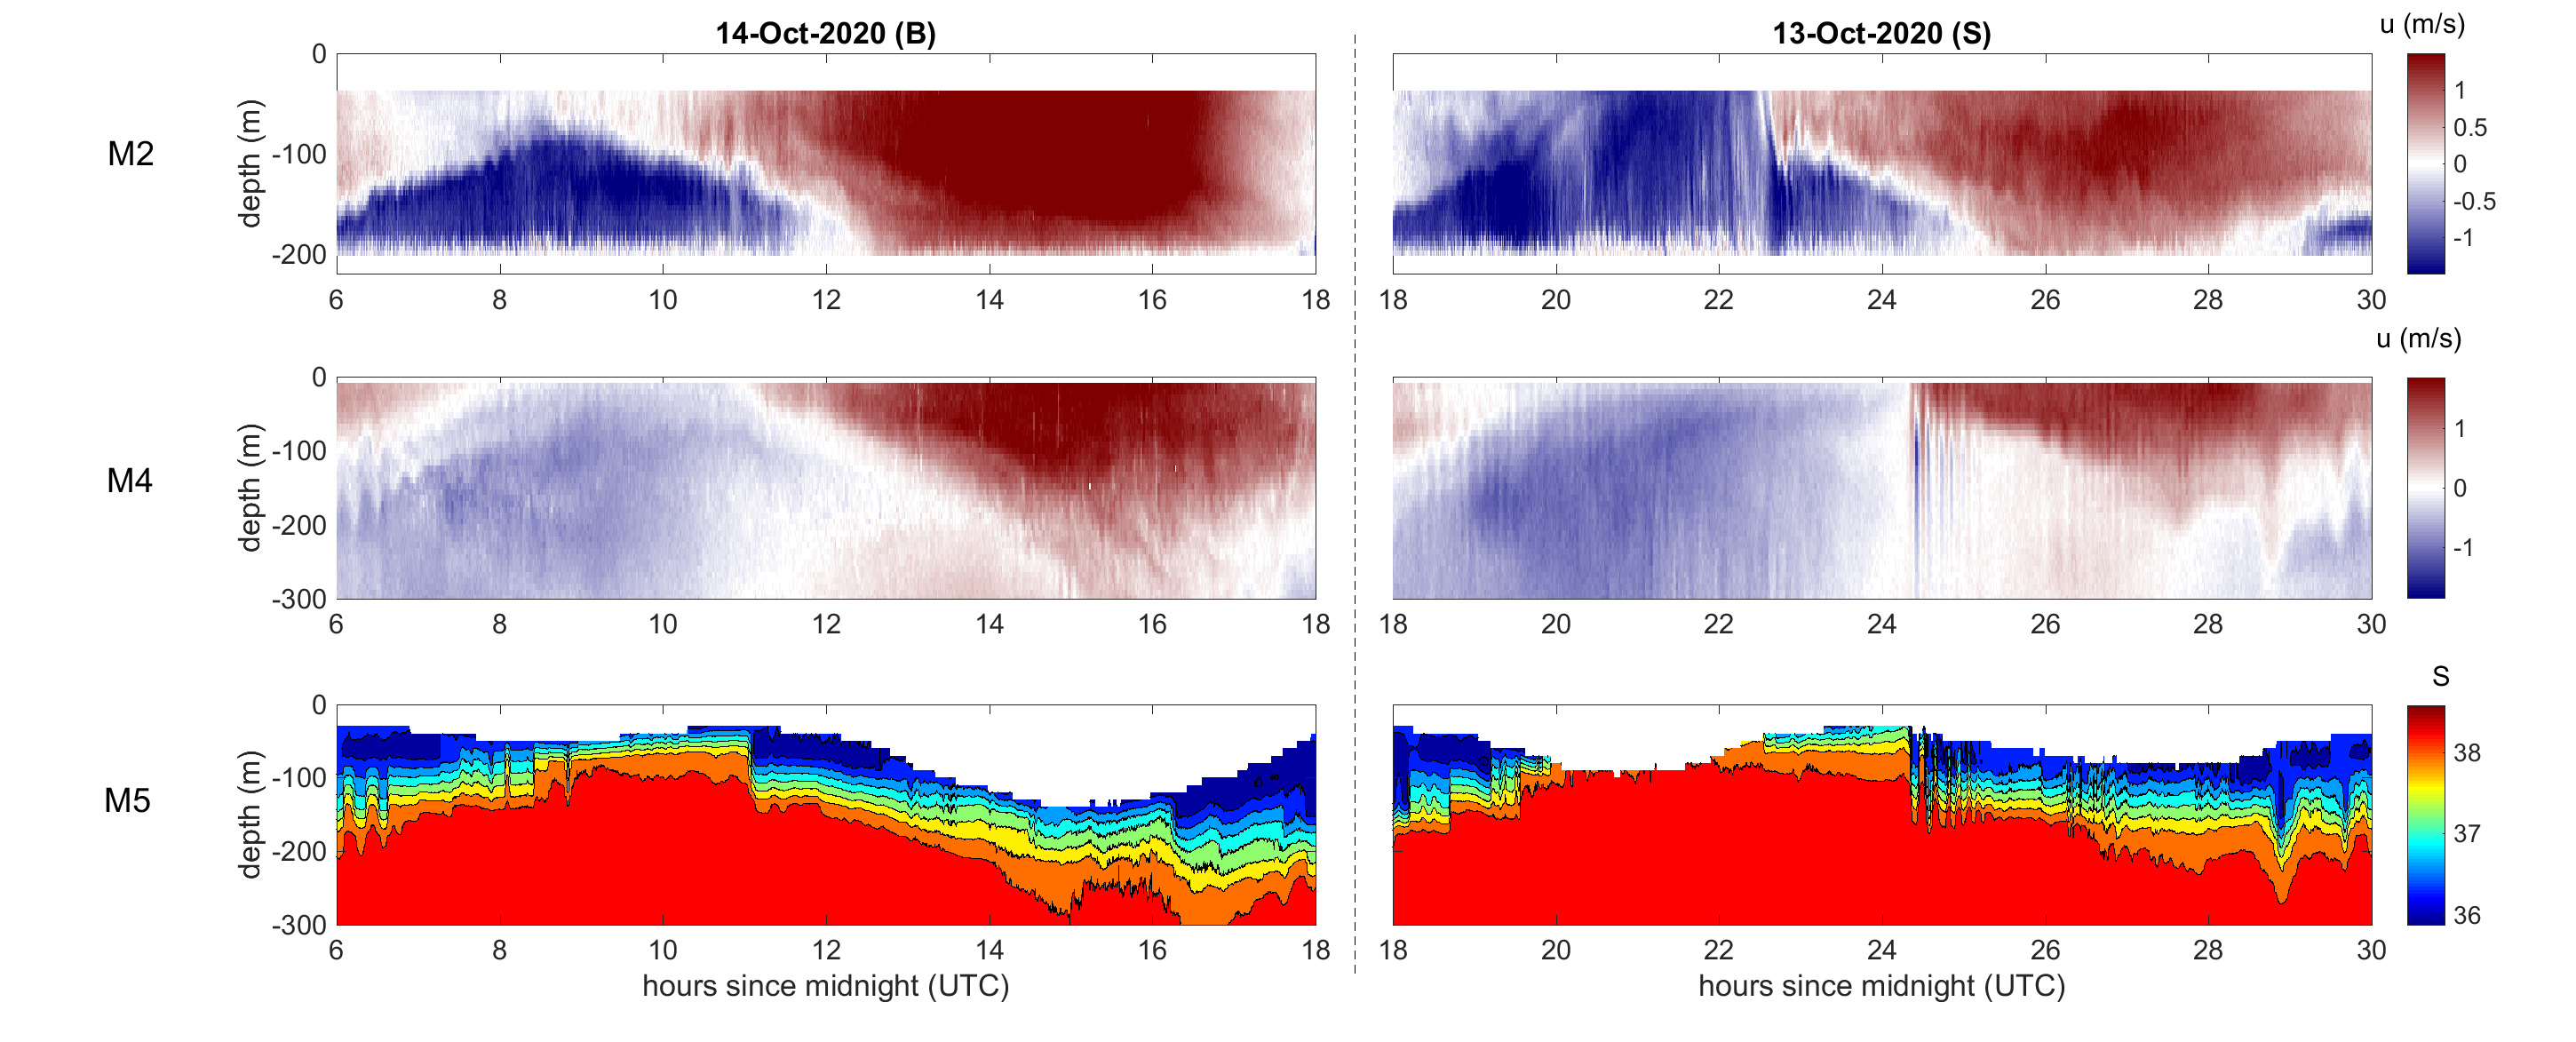
\includegraphics[width=\textwidth]{./GBR3D/US_moorings2.png}
 \caption {Same as \ref{fig_moor_US1} for a different time-period.}
 \label{fig_moor_US2}
\end{figure}

\begin{figure}[!h]
% \centering
 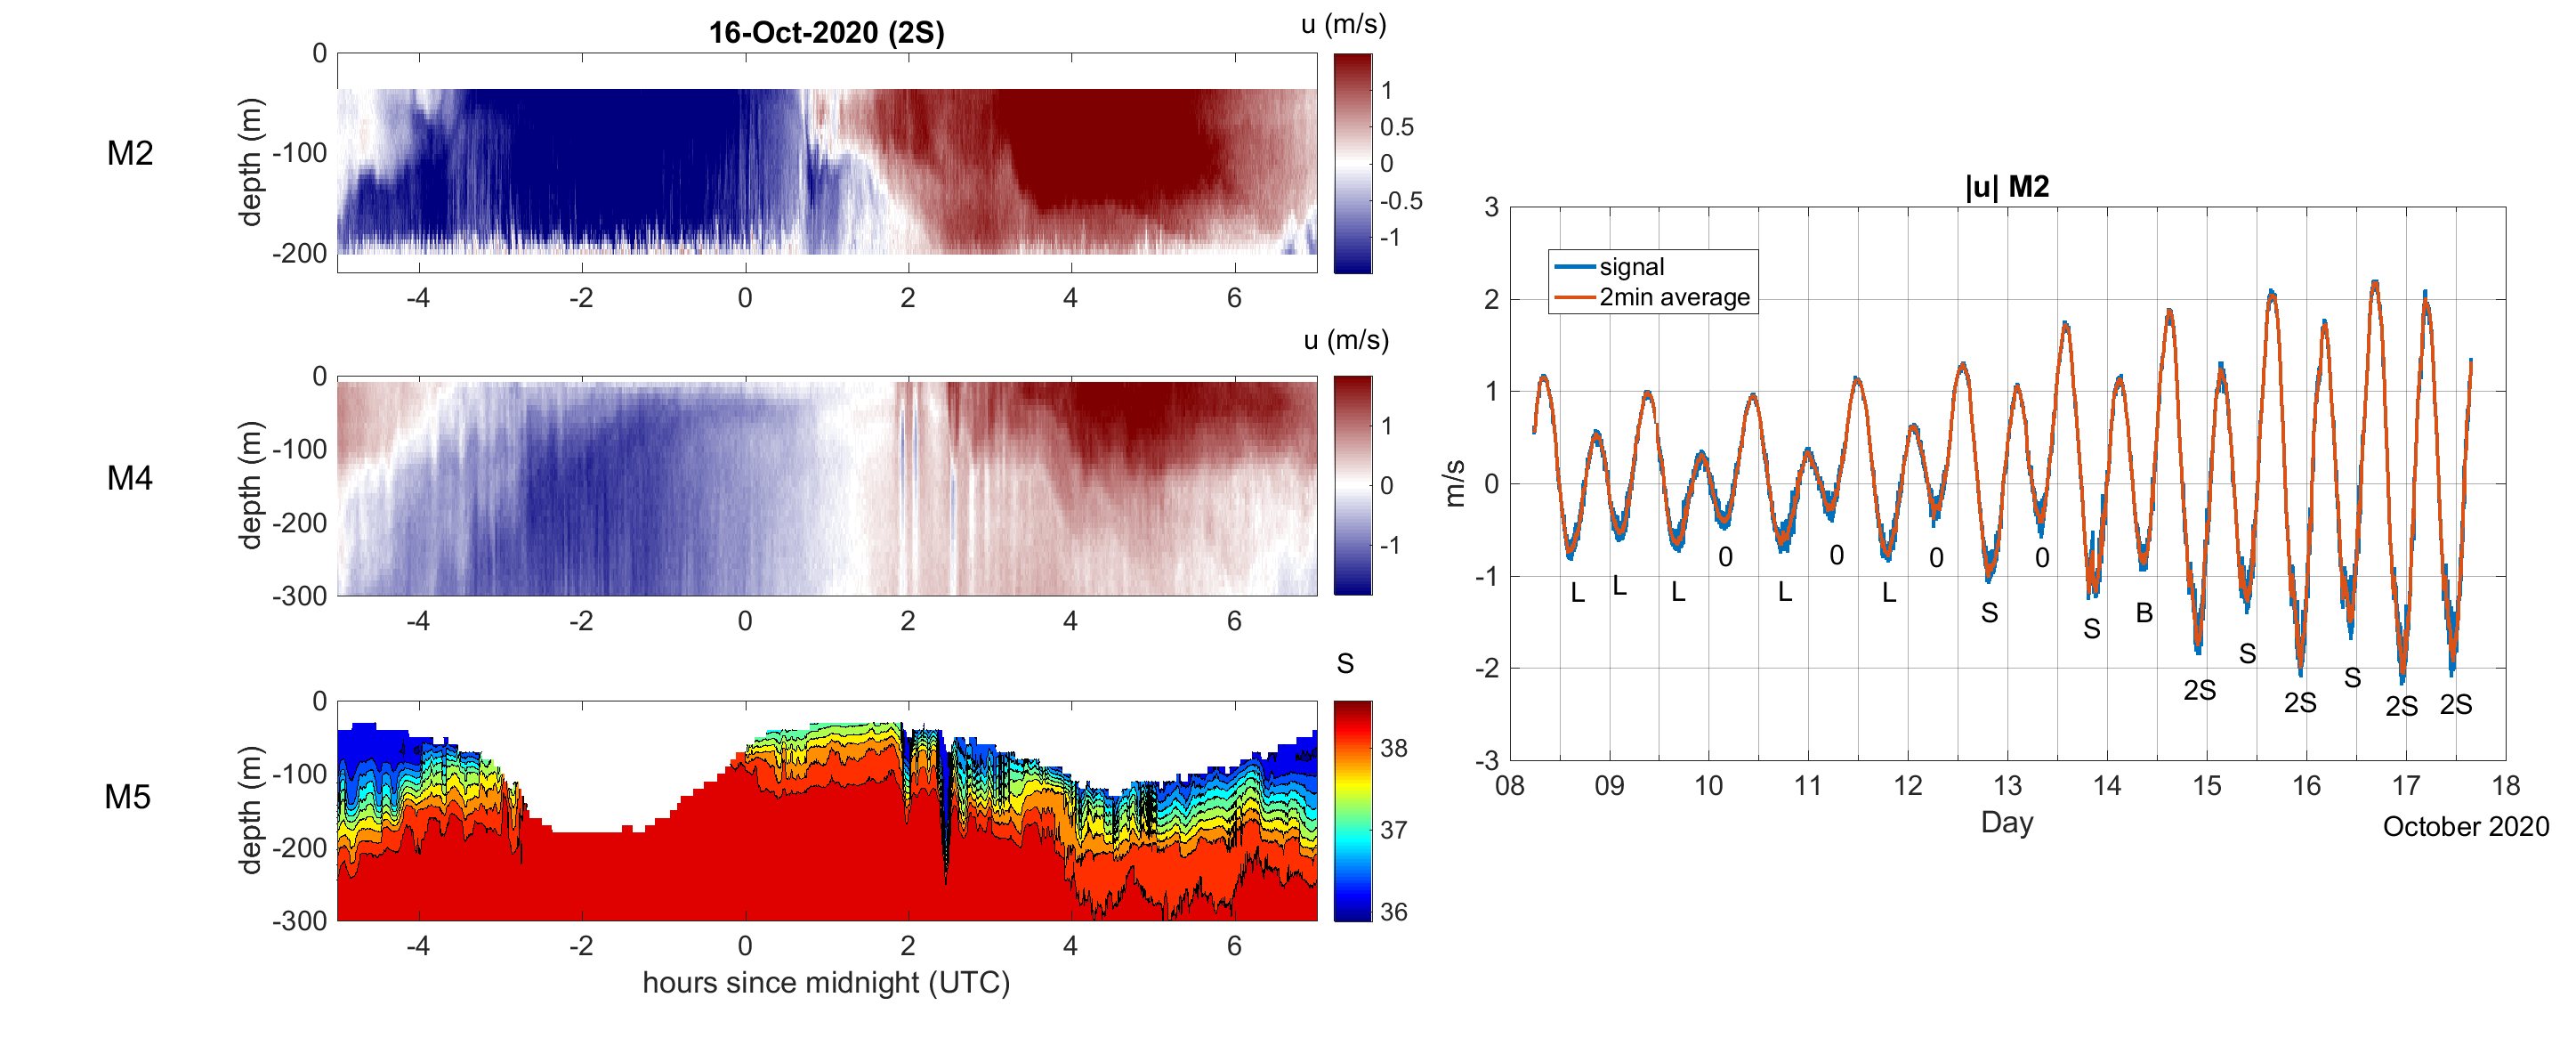
\includegraphics[width=\textwidth]{./GBR3D/US_moorings3.png}
 \caption {(a to c) Same as \ref{fig_moor_US1} for a different time-period. (d) Time-serie of depth-Averaged signal of zonal component of currents from M2 data. Each outflow is indicated the type of signal that is observed at M4 and M5.}
 \label{fig_moor_US3}
\end{figure}

Figures \ref{fig_moor_US1} to \ref{fig_moor_US3} (left part for the latter) present depth-time records of the zonal velocity (for M2 and M4 mooring) and salinity (for M5 mooring) for five different M2 tidal periods. Note that while all the water column is presented in those figures for the M2 data, only the upper 300m (of 500m total depth) are represented here for M4 and M5 data for better vizualisation.

Similarly, figure ... 
Figure ... presents the different signal at point near M4/M5 (just a bit west) in simulations SimST, SimNT and SimIT of section \ref{sectionSim3D}. This simulations are highly enough resolved that the train of solitary waves/bore can have devolved into a train of solitary waves by that point, and find the same types of signal except for the bore.


The currents at M2 . See that in inflow, always times when the whole water column flows eastward. In outflow time, either the flow becomes westward in the water column, as is the case in figure ..., or the baroclinic exchange situation holds with westward flow in the lower half and eastward currents in upper half of the water column, as is the case in ... . The latter case happens in neap-tide part of the forthnight cycle.

At M4, the whole inversion of the water column happens also for both outflow and inflow during the spring tide part of the cycle, although unlike at Camarinal still a shear area exist, that coincides with the interafce between mediterranean and atlantic water (see for exemple at 14H in 3 between 150-200mdepth). On this interface in M5 see signal of propagating internal gravity waves, sometimes accompagnied by 

First can see recurrent This is the case for a (ex at 3 hours in 2, 8h30 in 3, 19h30 in 4) this signal in M5 doesn't seem to be associated to a particular feature in the currents at M4. 

In ocntrast, another recurrent feature are the large amplitude troughs that can be seen during he 'inflow' part of the tidal cycle. Those later features are associated with a westward travelling train internal waves that is generated by reflection of the well-known eastward travelling internal wave train that is said to be generated at Camarinal Sill In this set it appears clearly in (29 in 4, ). 


But the focus is here made on the signal showing up at M4/M5 following the maximal outflow at M2, and associated to the depth-structure of currents at Camarinal Sill is like during the 'outflow' .

To understand, figure ... also gives exemple of the salinity and zinal velocity depth-time serie in the ... that were presented in section ... for four different ouflows. 

Depending on teh signal in the hours folloming the maximal outflow at M2, classification, (décrit sur obs, dit correspond dans sim et quel ressaut avant, etc):
\begin{itemize}
\item linear internal tide (o) : seen in figure ... where the depth of interface of density and velocity evolved linarly, during outflow upper layer still positive velocity
\item internal bore (b) : seen in figure ... , where see signal of travelling internal bore at M5 interface depth rapid evolution of 50(?)m, at M4 still see same linear evolution of velocity interface depth, at CS during outflow the upper layer velocity is near 0 or lightly negative. In the satellite SAR image in figure ... , corresponds to train of waves, the bore eventually devolves. In simulations not seen.
\item small amplitude wave (L) : seen in figure ... , where there is a signal that looks life internal waves of relatively small amplitude (10m) at M5, at M4 still linear evolution of the velocity interface. At M2, as with bore case velocity upper layer null or slightly negative. Sar image in ... shows after this outflow wave travelling in Alboran, only see trace of one wave.
\item Train of solitary waves (S) : two exemples are given, in figure ... and ...  see mode 1 signal at M4, succession of troughs at M5. at M2 in both case all captors of the water column find very negative current during outflow and abrupt return to two layer. The train of figure ... corresponds to the SAR image of figure ... of train exiting the strait. Train of figure ... corresponds to RGB(?) data on which can see a hydraulic jump. using notations of previous section, it is a w-jump.
\item Train of disorganized solitary waves (2S) : Seen in figures ... and ... (where no M4 data available at time of wave's passage). As previously whole negative signal of water column at M2. See disorganized train, in fact looks like two different train following each other. In figure (2) see linked to a previous w-jump. The two trains are for the two jumps at CS... (the main one on west of sill and the eats one...)
\end{itemize}
 (a) is just the internal tide witha linear evolution of the interface depth and currents, noted (o). (b) still see linear evolution of currents but small amplitude interanl waves are seen that seem somewhat non-linear (L). (c) is a packet of solitary waves with somewhat well arranged waves (S). (d) is several solitary waves, that look lifke two following train each with a great amplitude leading wave (2S)

 S and 2S signals are as expected linked to the jump at CS, however see an intermediate state that give L.

 In simIT, S signal can be seen , linked both times to an s-jump (western jump seen over the shallowest part of the Sill)
 SimST both time w-jump but the amplitude and proeminance of mode 1signature in current of the wave associated with the released eastern hydraulic jump can be small at M4/M5 in simulations, it depends on the northern reach of the hydraulic jump during outflow.  // In SimST, 2S signals although the first solitary wave that arrive(that would be linked to the eatsern jump) is low amplitude for first exemple, both are from w-jump, the difference is that the eastern jump in first case does not reach/extend as north in latitude, and could be confounded with S signal. 2nd has stronger barotropic currents at outflow // dire plutôt the amplitude of the first signal at this measure point will depend on the northern extent of the initial eastern jump.
 
 
In SimNT, see o and L signal. As expected, o smooth surface. However as was pointed in previous section, in simulations at least still can have wave in Alboran. Here L is linked previously to some disturbance of surface at CS though don't trigger the ... diagnosis. see a travelling wave. Also L here see the signal in velocity of mode 1.

This classification is applied to this first obseravtion period, and indicated in ... where see a pattern .


Arrive at neap tide part of the forthnight cycle and no solitons/nor signature of hydraulic jump are observed on moorings data until 11/10/2020 




Figure ... shows the four types of signal that are obserevd at M4 and M5, notations in figure ... indicate which type seen following the max outflow at CS. 



This subset of observations gives five distinct cases of set of observations between those two sites that is used to classify 

Note : classification S and 2S is very objective, S can expect that it's just both train have merged. they are linked to the form of the train. although hasn't seen on satellite an s-jump...  2S very distinct is for stronger tides, while S can be more regimes...






\begin{figure}[!h]
% \centering
 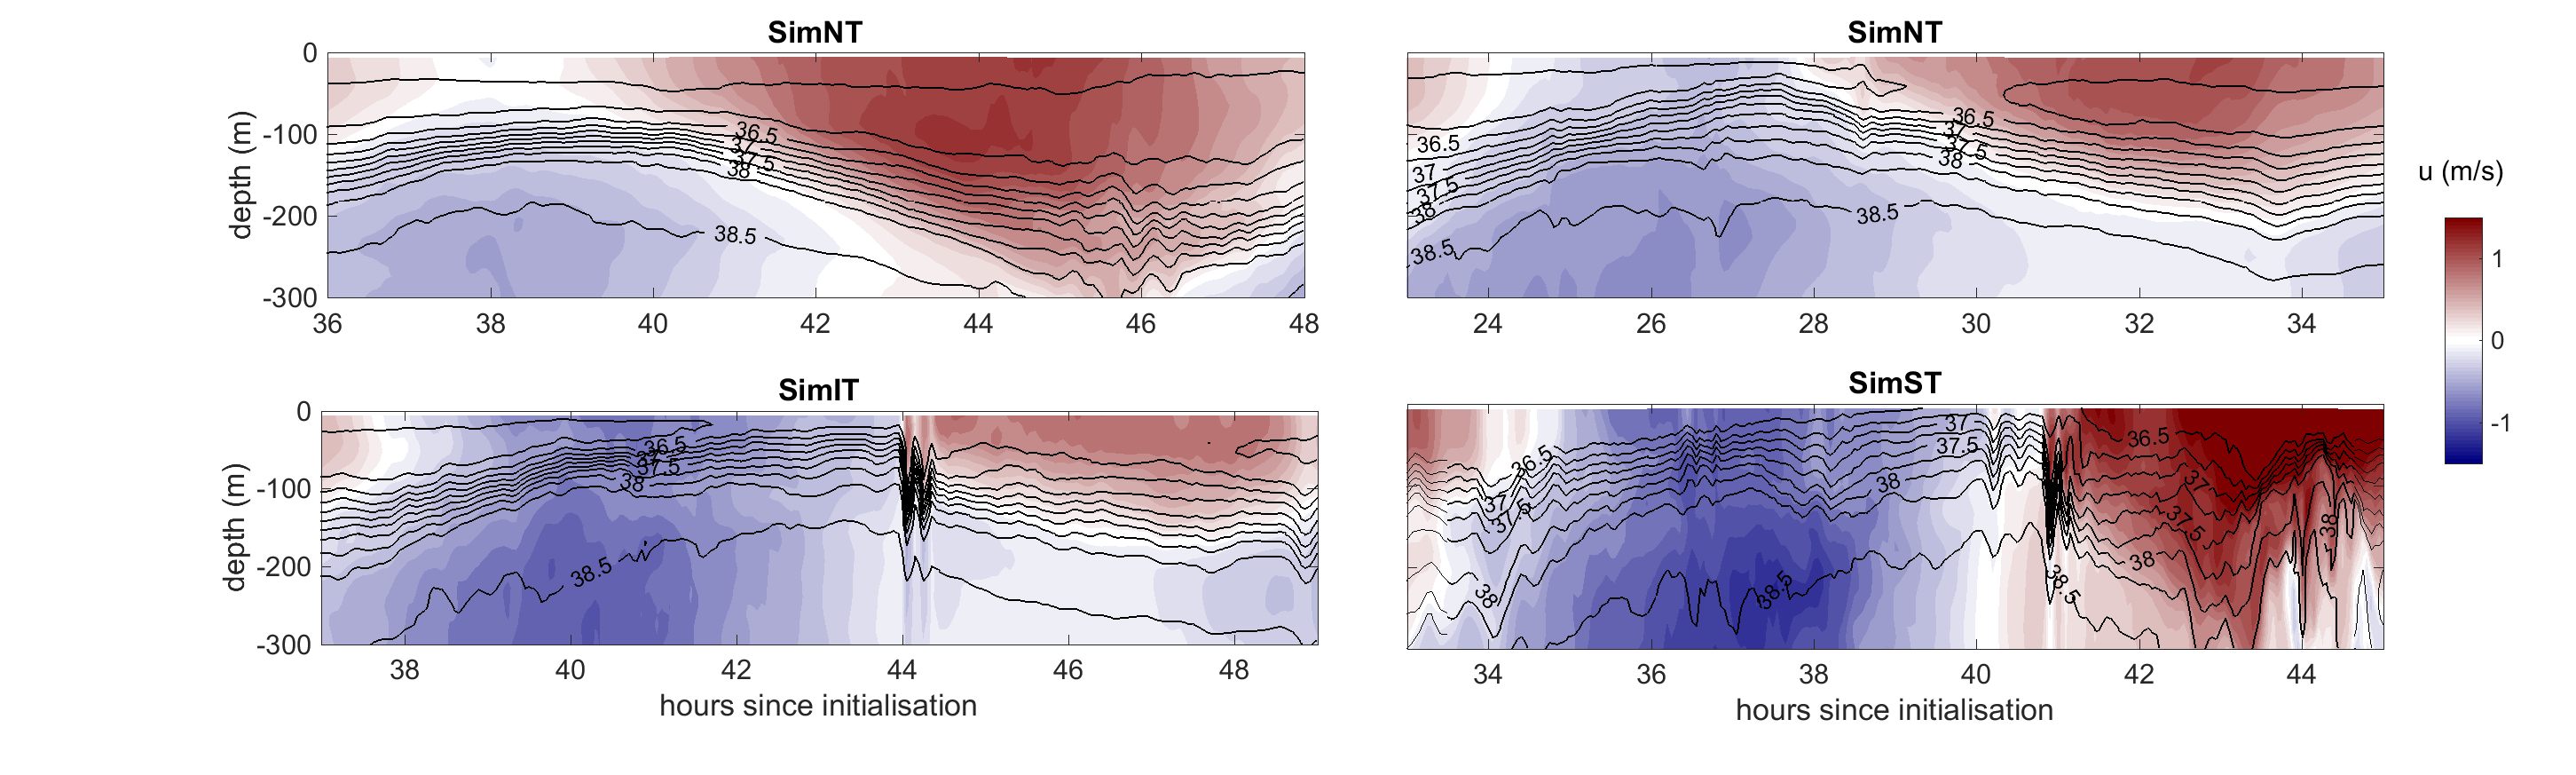
\includegraphics[width=\textwidth]{./GBR3D/US_M4SimMIV.png}
 \caption {Timesieries of salinity (black lines) and zonal velocity (colorbar) in the upper ... m in simulations ... Abscises is simulation time.}
 \label{Fig_moor_USs}
\end{figure}





%\subsubsection{Comparison with signal in 50m simulation}
%\label{section_sim_moor}

%This time can have surafce signature at CS for all this types of signals.

%Can also see maybe the signal at beginning of outflow / maybe the same.... comes from (???)







\subsection{Remarks on transition between regimens}

In figure (\noparref{fig_moor_US3}.2) are annoted the type of signal that is observed at M4/M5 after each corresponding outflow.

The first soliatry wave train detected at M4/M5 is the ... Before, only either low amplitude waves or only the internal tide signal of the interface. The next tidal cycle after this solitary wave, then. This is explained by the diurnal inequality


When look at the repartition of type of signals, see that L is more common than thought, and moreover when link to strength of barotropic current see evident link, since the hydraulic control conditions evolve.


Transitory regimens will be the hardest to medelise accurately. Accurate generation. Due to the sensiivity of the process

However, simulations showed that even if the train of solitary wave is not generated /may be generated even if there was no 


